% Loop Engineering vs Harness Engineering -- CVPR-style two-column technical report.
% Self-contained: builds with a standard TeX Live install (no external cvpr.sty needed).
% Build:  latexmk -pdf loop-engineering.tex      (or: pdflatex x2)
\documentclass[10pt,twocolumn,letterpaper]{article}

\usepackage[T1]{fontenc}
\usepackage[utf8]{inputenc}
\usepackage{times}
\usepackage[letterpaper,left=0.8125in,right=0.8125in,top=1in,bottom=1in,columnsep=0.3125in]{geometry}
\usepackage{graphicx}
\usepackage{amsmath,amssymb}
\usepackage{booktabs}
\usepackage{array}
\usepackage{xcolor}
\usepackage{listings}
\usepackage{caption}
\usepackage{enumitem}
\usepackage{url}
\usepackage{tikz}
\usetikzlibrary{positioning,arrows.meta,calc,fit,backgrounds,shapes.geometric}
\usepackage[hidelinks]{hyperref}

% --- CVPR-ish section styling -------------------------------------------------
\usepackage{titlesec}
\titleformat{\section}{\normalfont\large\bfseries}{\thesection.}{0.5em}{}
\titleformat{\subsection}{\normalfont\normalsize\bfseries}{\thesubsection.}{0.5em}{}
\setlength{\parskip}{0pt}
\captionsetup{font=small,labelfont=bf}

% --- listings style for pseudo-code / shell ----------------------------------
\definecolor{codebg}{rgb}{0.96,0.96,0.96}
\lstset{
  basicstyle=\ttfamily\footnotesize,
  backgroundcolor=\color{codebg},
  breaklines=true,
  columns=fullflexible,
  keepspaces=true,
  frame=single,
  framesep=4pt,
  xleftmargin=4pt,
  aboveskip=6pt,
  belowskip=6pt,
}

\newcommand{\Lset}{\ensuremath{L}}
\newcommand{\Hset}{\ensuremath{H}}

\begin{document}

% =============================== TITLE + ABSTRACT (full width) ================
\twocolumn[{%
\centering
{\LARGE \bfseries Loop Engineering and Harness Engineering: A Comparative\\[2pt]
Analysis of Two Disciplines for Operating Autonomous Coding Agents \par}
\vspace{1.2em}
{\large Duy Tran Thanh \par}
\vspace{0.4em}
{\normalsize \texttt{duy.tran10@onemount.com} \par}
\vspace{1.6em}
\begin{minipage}{0.92\textwidth}
\begin{center}\textbf{Abstract}\end{center}
\itshape
The rapid capability gains of large language model (LLM) coding agents have
shifted the locus of engineering effort away from the model and toward the
system that operates it. Two named disciplines emerged in 2026: \emph{loop
engineering}, the design of the self-running cycle that prompts an agent toward
a goal, and \emph{harness engineering}, the design of the full scaffolding that
surrounds a model to make it reliable. The two are frequently conflated. This
report formalizes both, argues that they stand in a part--whole relation rather
than competing, and characterizes the distinct failure modes each addresses. We
give a six-tuple formal model of a loop, identify two safety invariants
(mandatory verification, mandatory termination) that distinguish an engineered
loop from the colloquial ``Ralph loop,'' and ground the analysis in OnLOOP, a
contracts-first reference implementation. We conclude that loop engineering is
the temporal/control-flow specialization of harness engineering, and that the
chief practical contribution of treating the loop as a first-class object is the
promotion of verification and termination from discretionary practices to
type-level obligations.
\vspace{1.4em}
\end{minipage}
}]

% =============================== OVERVIEW FIGURE (teaser) =====================
\begin{figure*}[t]
\centering
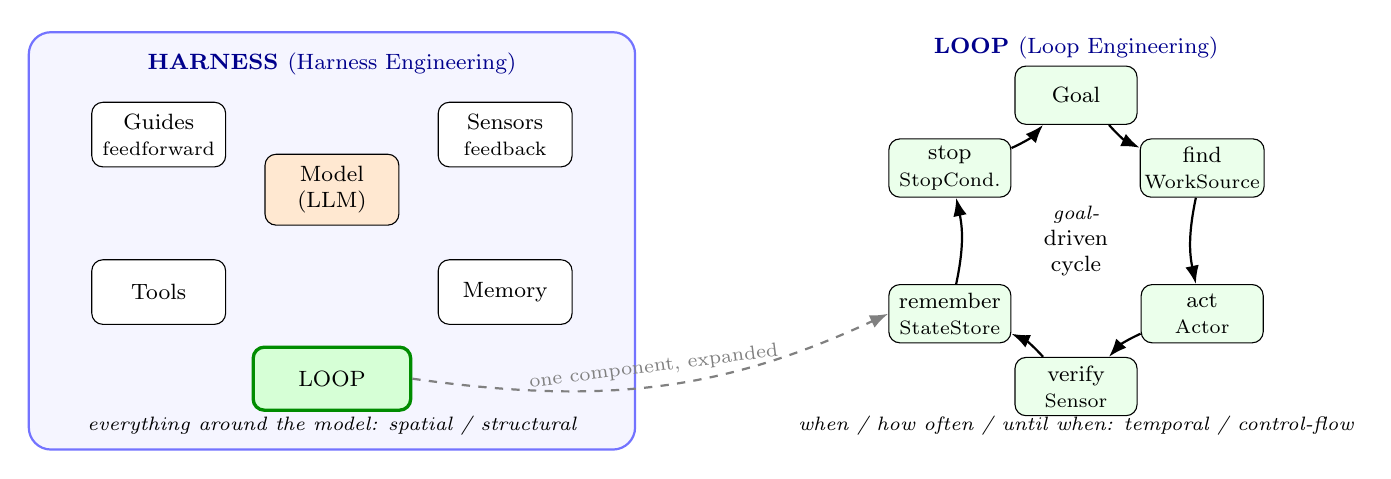
\begin{tikzpicture}[
  font=\footnotesize, >=Latex,
  comp/.style={draw, rounded corners, fill=white, align=center, minimum width=1.7cm, minimum height=0.82cm, inner sep=2pt},
  modelnode/.style={draw, fill=orange!18, rounded corners, align=center, minimum width=1.7cm, minimum height=0.9cm},
  loopnode/.style={draw=green!55!black, very thick, fill=green!16, rounded corners, align=center, minimum width=2.0cm, minimum height=0.8cm},
  ring/.style={draw, fill=green!8, rounded corners, align=center, minimum width=1.55cm, minimum height=0.74cm, inner sep=1.5pt},
]
% ---------- LEFT: the harness (spatial) ----------
\draw[rounded corners=8pt, fill=blue!4, draw=blue!55, thick] (-0.4,-2.95) rectangle (7.3,2.35);
\node[blue!55!black] at (3.45,1.95) {\bfseries HARNESS \textnormal{(Harness Engineering)}};
\node[modelnode] (model)  at (3.45,0.35) {Model\\(LLM)};
\node[comp] (guides)  at (1.25,1.05)  {Guides\\{\scriptsize feedforward}};
\node[comp] (sensors) at (5.65,1.05)  {Sensors\\{\scriptsize feedback}};
\node[comp] (tools)   at (1.25,-0.95) {Tools};
\node[comp] (memory)  at (5.65,-0.95) {Memory};
\node[loopnode] (loopbox) at (3.45,-2.05) {LOOP};
\node[align=center] at (3.45,-2.65) {\scriptsize\itshape everything around the model: spatial / structural};

% ---------- RIGHT: the loop cycle (temporal) ----------
\def\cx{12.9}\def\cy{-0.30}
\node[blue!55!black] at (\cx,2.15) {\bfseries LOOP \textnormal{(Loop Engineering)}};
\node[ring] (g) at ($(\cx,\cy)+(90:1.85)$)   {Goal};
\node[ring] (w) at ($(\cx,\cy)+(30:1.85)$)   {find\\{\scriptsize WorkSource}};
\node[ring] (a) at ($(\cx,\cy)+(-30:1.85)$)  {act\\{\scriptsize Actor}};
\node[ring] (s) at ($(\cx,\cy)+(-90:1.85)$)  {verify\\{\scriptsize Sensor}};
\node[ring] (m) at ($(\cx,\cy)+(-150:1.85)$) {remember\\{\scriptsize StateStore}};
\node[ring] (t) at ($(\cx,\cy)+(150:1.85)$)  {stop\\{\scriptsize StopCond.}};
\node[align=center] at (\cx,\cy) {\scriptsize\itshape goal-\\driven\\cycle};
\draw[->,thick] (g) to[bend right=12] (w);
\draw[->,thick] (w) to[bend right=12] (a);
\draw[->,thick] (a) to[bend right=12] (s);
\draw[->,thick] (s) to[bend right=12] (m);
\draw[->,thick] (m) to[bend right=12] (t);
\draw[->,thick] (t) to[bend right=12] (g);
\node[align=center] at (\cx,-2.65) {\scriptsize\itshape when / how often / until when: temporal / control-flow};

% ---------- LINK: the loop is one component of the harness ----------
\draw[dashed,->,thick,gray] (loopbox.east) to[out=-8,in=205]
  node[midway,above,sloped]{\scriptsize one component, expanded} (m.west);
\end{tikzpicture}
\caption{\textbf{Overview: harness engineering vs.\ loop engineering.}
\emph{Left:} the harness is everything around the model---guides (feedforward),
sensors (feedback), tools, memory, and the loop---engineered along a
\emph{spatial} axis (what surrounds the model). \emph{Right:} the loop is one
component of the harness, shown expanded; loop engineering designs its
\emph{temporal} cycle Goal\,$\to$\,find\,$\to$\,act\,$\to$\,verify\,$\to$\,
remember\,$\to$\,stop, and owns termination. The two disciplines are a part and
a whole, not rivals: harness engineering draws the box; loop engineering
animates one part of it over time ($L \subsetneq H$).}
\label{fig:overview}
\end{figure*}

% =============================== 1. INTRODUCTION =============================
\section{Introduction}
A coding agent is increasingly described by the decomposition
$\mathrm{Agent} = \mathrm{Model} + \mathrm{Harness}$, where the \emph{model}
supplies intelligence and the \emph{harness} is ``everything in an AI agent
except the model itself''~\cite{bockeler,osmaniharness}. As frontier models
saturate single-prompt benchmarks, the marginal return on prompt-level
optimization falls and the return on system-level design rises. Two disciplines
name this system-level work; Fig.~\ref{fig:overview} previews how they differ.

\textbf{Loop engineering} is ``building a system that prompts your agent on a
schedule and against a goal, instead of typing each prompt
yourself''~\cite{osmaniloop}. Its thesis: leverage has moved from the quality of
a single prompt to the design of the system that \emph{generates and verifies}
prompts.

\textbf{Harness engineering} is ``the discipline of designing, building, and
iterating on the scaffolding that surrounds a language
model''~\cite{bockeler}: context delivery, tool interfaces, guardrails, memory,
sandboxes, and feedback loops.

Practitioners often use the terms interchangeably, or treat them as rival
schools. We argue this is a category error and make four contributions:
(1) a formal six-tuple model of an engineered loop and its execution semantics
(Sec.~\ref{sec:loop}); (2) a characterization of harness engineering as a
feedforward/feedback control structure, with a proof-sketch that the loop is a
proper subcomponent of the harness (Sec.~\ref{sec:harness}); (3) a
multi-dimensional comparison establishing that the disciplines optimize
orthogonal axes (Sec.~\ref{sec:compare}); and (4) an empirical grounding in
OnLOOP, whose type system enforces two invariants that the bare Ralph loop
leaves optional (Sec.~\ref{sec:onloop}).

% =============================== 2. BACKGROUND ==============================
\section{Background and Related Work}

\subsection{The agent loop}
The cyclic structure of a rational agent (perceive, deliberate, act, observe)
predates LLMs by decades. It is the basic control structure of the
Belief--Desire--Intention model and is codified in standard
textbooks~\cite{russellnorvig}. LLMs did not invent the loop; they made a
general-purpose actor cheap enough to place inside it, which unlocked open-ended
agentic behavior~\cite{oracle}.

\subsection{Loop engineering and the Ralph loop}
The phrase \emph{loop engineering} was popularized by Osmani~\cite{osmaniloop}
in June 2026, crystallizing observations by Steinberger (``you should be
designing loops that prompt your agents'') and Cherny (``my role shifted to
write loops rather than to prompt the model directly''). Its minimal
instantiation is the \textbf{Ralph loop}~\cite{ralph}, whose canonical form is
one line:
\begin{lstlisting}[language=bash]
while :; do cat PROMPT.md | agent ; done
\end{lstlisting}
Its insight is that progress lives in files and git history, not in the context
window: each iteration starts a fresh agent with a fixed prompt, does a little
work, writes results to disk, and exits. The convention separates a fixed task
(\texttt{PROMPT.md}), accumulated learnings (\texttt{AGENTS.md}), and a progress
log (\texttt{progress.md})~\cite{ralph,bharath}. Critically, the bare Ralph loop
has \emph{no required verifier and no termination condition}; the
\texttt{while :;} is literally infinite. We return to this in
Sec.~\ref{sec:onloop}.

\subsection{Harness engineering}
\emph{Harness engineering} was developed by B\"ockeler~\cite{bockeler} at
Thoughtworks and elaborated by Osmani~\cite{osmaniharness} and
LangChain~\cite{langchain}. It frames the harness as two classes of control:
\emph{feedforward} guides (conventions, documentation, templates, linters set
ahead of time) and \emph{feedback} sensors (tests, static analysis, review
agents that observe output and enable self-correction). LangChain reports that
an explicit four-stage structure (Plan, Build, Verify, Fix) outperforms
unstructured loops~\cite{langchain}, evidence that harness structure, not raw
model capability, governs reliability.

% =============================== 3. DEFINITIONS =============================
\section{Definitions}
We fix terminology. The \textbf{model} ($M$) is the LLM, a black-box stochastic
function from context to text/tool-calls. The \textbf{harness} ($H$) is the
deterministic-and-inferential system around $M$; everything that is not $M$. The
\textbf{loop} ($L$) is the control structure that repeatedly invokes the agent
toward a goal; a component of $H$. A \textbf{sensor} observes an action's result
and returns a verdict with evidence (feedback). A \textbf{guide} constrains
generation before it occurs (feedforward).

% =============================== 4. LOOP MODEL ==============================
\section{A Formal Model of Loop Engineering}
\label{sec:loop}

\subsection{The loop as a six-tuple}
We model an engineered loop as $\Lset = (G, W, A, S, M_s, T)$, with components
given in Table~\ref{tab:tuple}.

\subsection{Inputs and outputs}
Readers reasonably ask what loop engineering \emph{consumes} and \emph{produces}.
Viewed as a function, a loop has the signature
\[
\texttt{run}:\;
\underbrace{(G,W,A,S,M_s,T)}_{\text{config}}\times
\underbrace{(\mathsf{Wksp}, M, \mathsf{Budget})}_{\text{environment}}
\;\to\;
\underbrace{(r, D, \sigma^{\ast}, \mathcal{H}, \mathsf{Wksp}')}_{\text{outcome}}
\]
summarized in Fig.~\ref{fig:io}. The \textbf{input} is, in one phrase, \emph{a
goal plus the means to pursue and check it}: the objective $G$ with its success
predicate, the model $M$ as the actor's oracle, the workspace $\mathsf{Wksp}$ to
act on, any state $\sigma_0$ restored from a prior run (so a loop resumes rather
than restarts), and the verification/termination policy ($S$, $T$, budget). The
\textbf{output} is \emph{a terminated, audited outcome}: a stop reason $r$; a
done-set $D$ containing only items that passed their sensors (by P1); the
mutated work product $\mathsf{Wksp}'$ on disk; a replayable per-iteration trace
$\mathcal{H}$; and a final state $\sigma^{\ast}$ that is itself a valid input to
the next run. The output is thus \emph{self-describing} (why it stopped),
\emph{verifiable} (what passed), and \emph{resumable} (where to continue). This
contrasts with harness engineering, whose I/O is per-\emph{step}: it maps a
model plus task context (guides, tools, memory) to one constrained,
sensor-checked action. A loop's I/O is the closure of the harness's I/O over
many steps until $T$ fires.

\begin{figure}[t]
\centering
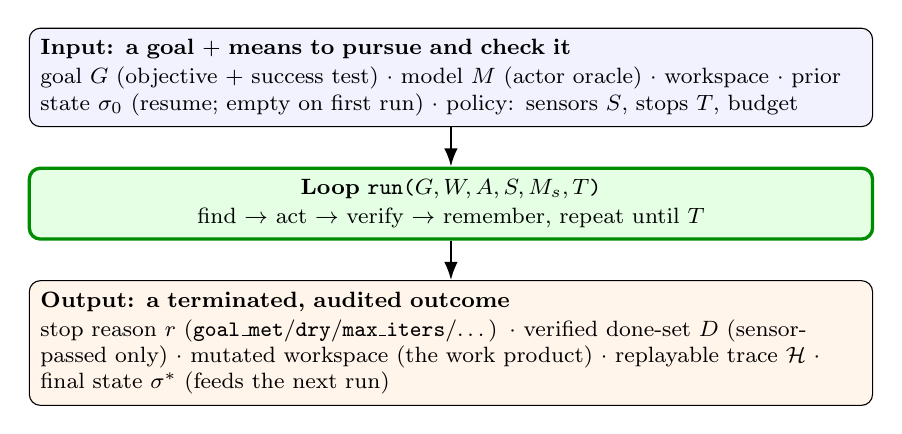
\begin{tikzpicture}[font=\footnotesize, >=Latex, node distance=5mm,
  io/.style={draw, rounded corners, align=left, text width=0.86\columnwidth, inner sep=4pt},
  run/.style={draw, very thick, draw=green!55!black, rounded corners, fill=green!10, align=center, text width=0.86\columnwidth, inner sep=4pt}]
\node[io, fill=blue!5] (in) {\textbf{Input: a goal $+$ means to pursue and check it}\\[1pt]
goal $G$ (objective $+$ success test) $\cdot$ model $M$ (actor oracle) $\cdot$
workspace $\cdot$ prior state $\sigma_0$ (resume; empty on first run) $\cdot$
policy: sensors $S$, stops $T$, budget};
\node[run, below=of in] (run) {\textbf{Loop} \texttt{run(}$G,W,A,S,M_s,T$\texttt{)}\\[1pt]
find $\to$ act $\to$ verify $\to$ remember, repeat until $T$};
\node[io, fill=orange!8, below=of run] (out) {\textbf{Output: a terminated, audited outcome}\\[1pt]
stop reason $r$ (\texttt{goal\_met}/\texttt{dry}/\texttt{max\_iters}/\dots) $\cdot$
verified done-set $D$ (sensor-passed only) $\cdot$ mutated workspace (the work
product) $\cdot$ replayable trace $\mathcal{H}$ $\cdot$ final state $\sigma^{\ast}$
(feeds the next run)};
\draw[->,thick] (in) -- (run);
\draw[->,thick] (run) -- (out);
\end{tikzpicture}
\caption{Inputs and outputs of a loop. Loop engineering turns a \emph{goal}
(plus a model oracle, a workspace, and a verification/termination policy) into a
\emph{terminated, verified outcome} whose final state is a valid input to the
next run.}
\label{fig:io}
\end{figure}

\subsection{Execution semantics}
A run is generated by applying the transition rule of Fig.~\ref{fig:rule} from an
initial state $\sigma_0$ loaded from $M_s$. The timestamp $\tau$ is supplied by
the runtime, not read by any contract, which keeps a run replayable from its
recorded trace.

\subsection{Properties}
Two properties follow directly and are the heart of the discipline.
\begin{itemize}[leftmargin=1.2em,itemsep=2pt,topsep=2pt]
\item \textbf{P1 (Verified progress).} By rules (R2)--(R3), an item enters the
done-set only if the conjunction of all sensors passes. No sensor, no progress:
an action the loop cannot check does not advance the goal.
\item \textbf{P2 (Guaranteed termination).} If $T$ contains at least one bound
monotone in a quantity the runtime increments every pass (iterations,
accumulated cost, or consecutive empty rounds), the run halts. Rule (R1)
evaluates $T$ before any work, so the bound cannot be skipped.
\end{itemize}
P1 and P2 are not automatic; they hold only if $S \neq \emptyset$ and $T$
contains a real bound. An \emph{engineered} loop is precisely one in which these
are obligations rather than options (Sec.~\ref{sec:onloop}).

\subsection{Patterns as instances of \texorpdfstring{$L$}{L}}
Common patterns are recovered by choosing components, not by writing new control
flow: the \emph{Ralph loop} fixes $G$ to a spec, sets $M_s$ to files+git, and
leaves $S,T$ empty (its weakness); \emph{loop-until-dry} puts a $k$-empty-round
bound in $T$; \emph{fan-out/verify} lets $W$ yield independent items under
isolation; \emph{adversarial verify} makes $S$ a panel whose verdict requires a
majority to survive refutation.

% =============================== 5. HARNESS MODEL ==========================
\section{A Formal View of Harness Engineering}
\label{sec:harness}

\subsection{The harness as a control structure}
Following B\"ockeler~\cite{bockeler}, the harness is a pair of control
populations over the model, $H = (\mathit{Guides}, \mathit{Sensors},
\mathit{Tools}, \mathit{Memory}, L)$, where \emph{Guides} are feedforward and
\emph{Sensors} are feedback. The central operating rule is a \emph{meta-loop}:
whenever an issue recurs, the feedforward and feedback controls are improved.
This is a second-order loop in which the engineer (or, prospectively, an
automated guide-writer) updates $\mathit{Guides}$ and $\mathit{Sensors}$ in
response to recurring failures.

\subsection{The loop is a subcomponent of the harness}
\noindent\textbf{Proposition.} $L \subsetneq H$.

\noindent\emph{Argument.} The harness is defined as everything that is not the
model. The loop's components $W, A, S, M_s, T$ are each non-model procedures,
hence elements of $H$. The loop's sensors $S$ are exactly the feedback-control
population; its memory $M_s$ is the harness memory; its actor $A$ is the
harness's invocation of the model. The loop additionally contributes control
flow ($T$ and the transition rule) that the static harness does not. Conversely
$H$ contains $\mathit{Guides}$ and $\mathit{Tools}$ outside the loop's defining
tuple. Hence $L \subsetneq H$. \hfill$\square$

This is the central structural claim: \emph{loop engineering is the control-flow
specialization of harness engineering.} They are not rivals; one is part of the
other.

\subsection{Two loops, often conflated}
There are two distinct cycles: the \emph{inner agent loop} (perceive--act
--verify), a harness component formalized as $L$; and the \emph{outer steering
loop}, B\"ockeler's meta-loop, in which a human improves guides and sensors over
time. Loop engineering, in its strong form, is partly the project of automating
the outer loop (e.g., appending learnings to \texttt{AGENTS.md}) so supervision
scales sublinearly with agent activity.

% =============================== 6. COMPARISON =============================
\section{Comparative Analysis}
\label{sec:compare}
We compare along ten dimensions, summarized in Table~\ref{tab:compare}.

\subsection{Object and axis (orthogonality)}
The cleanest distinction is \emph{axis}. Harness engineering operates on a
\emph{spatial} axis: breadth of scaffolding around the model at one instant.
Loop engineering operates on a \emph{temporal} axis: cadence and control flow
across many invocations. One can improve the harness (a linter, a better
template) without changing the loop, and change the loop (schedule it, add
loop-until-dry) without changing the guides. Orthogonality is the operational
signature that two disciplines are distinct rather than synonymous.

\subsection{Failure mode (the diagnostic test)}
Reach for \emph{harness} vocabulary when the symptom is ``the agent produces
wrong or unconstrained output''; the fix is in guides and sensors. Reach for
\emph{loop} vocabulary when the symptom is ``the agent is capable, but I am
stuck driving every iteration''; the fix is a scheduled, goal-driven,
self-verifying cycle.

\subsection{Verification and termination}
Both disciplines centre verification, which is why they are easy to conflate:
they refer to the same artifacts (tests, linters, review agents) under different
framings, a static taxonomy of controls versus a stage in a dynamic cycle.
\emph{Termination}, by contrast, is owned by loop engineering and largely
ignored by harness engineering: a static harness has no notion of when to stop.
Property P2 and the obligation $T \neq \emptyset$ only make sense once the loop
is a first-class object.

% =============================== 7. CASE STUDY ============================
\section{Case Study: OnLOOP}
\label{sec:onloop}
OnLOOP is a contracts-first reference implementation: an existence proof that the
formal model is realizable and that the safety invariants can be enforced
mechanically.

\subsection{Architecture}
OnLOOP implements the six-tuple as six abstract interfaces (\texttt{Goal},
\texttt{WorkSource}, \texttt{Actor}, \texttt{Sensor}, \texttt{StateStore},
\texttt{StopCondition}). A concrete loop is one implementation of each, declared
in a YAML spec that binds a contract to a class via a dotted path. A runtime
executes the rule of Fig.~\ref{fig:rule}: stop conditions are checked first
(R1), progress requires all sensors to pass (R2--R3), and state is persisted
every pass (R4) through a JSON \texttt{StateStore}, making runs restartable.

\subsection{Invariants as type-level obligations}
OnLOOP's spec schema enforces P1 and P2 \emph{at load time}: \texttt{sensors}
requires at least one entry (a loop that cannot check itself will not load,
enforcing $S \neq \emptyset$), and \texttt{stop} requires at least one entry (a
loop that cannot terminate will not load, enforcing $T \neq \emptyset$). This is
the report's main practical claim: the value of treating the loop as a
first-class object is the promotion of verification and termination from
optional practices to non-negotiable, machine-checked obligations.

\subsection{The Ralph loop as a degenerate instance}
In the model of Sec.~\ref{sec:loop}, the bare Ralph loop is the instance with
$S = \emptyset$ and $T = \emptyset$. Both safety properties fail. OnLOOP rejects
exactly this configuration:
\begin{quote}\itshape
The Ralph loop is the loop with the brakes optional. OnLOOP is the same loop
with the brakes required.
\end{quote}

\subsection{Empirical sanity check}
A deterministic, model-free reference loop (clearing a punch list on disk)
exercises every component and each stop reason. Its end-to-end suite confirms:
convergence to \texttt{goal\_met} with verified progress; correct bounding by
\texttt{max\_iters} before goal; \texttt{loop\_until\_dry} termination on an empty
work source; that a permanently failing sensor blocks an item from the done-set
(a direct test of P1); and that state round-trips across a simulated restart (a
test of R4). All cases pass. Because the actor is deterministic, the suite
isolates the control structure from model stochasticity, which is the property
under test. We make no claim about model-in-the-loop performance; that is future
work.

% =============================== 8. DISCUSSION ===========================
\section{Discussion}
Fig.~\ref{fig:nest} gives the unifying picture: harness engineering draws the
box; loop engineering animates one component of it over time. The disciplines
are complementary and a mature system needs both. A reasonable order of
operations: establish a harness with at least one feedback sensor and a useful
guide; then engineer the loop that drives the agent through it, fixing
termination and verification first because they are the cheap, high-consequence
invariants. Conflating the two yields two characteristic mistakes: treating loop
engineering as the whole story gives the Ralph failure (a slick autonomous cycle
with no brakes); treating harness engineering as the whole story gives a
well-instrumented agent that still needs a human in the chair for every step.

% =============================== 9. LIMITATIONS ==========================
\section{Limitations and Threats to Validity}
\textbf{Construct validity:} both terms are recent (2026) and not standardized;
our definitions follow the originating sources but usage is in flux.
\textbf{Single implementation:} our grounding is one framework with a
deterministic actor; we show the invariants are enforceable and the control
structure correct, not that LLM-actor loops converge efficiently on real tasks.
\textbf{No model-in-the-loop benchmark:} we deliberately exclude model
stochasticity to isolate control flow, so we report no task-success or cost
metrics; the LangChain result~\cite{langchain} is cited as external evidence,
not our measurement. \textbf{Generality:} the claim $L \subsetneq H$ rests on
the ``everything but the model'' definition of harness.

% =============================== 10. CONCLUSION ==========================
\section{Conclusion and Future Work}
Loop engineering and harness engineering are a part and a whole. The harness is
the spatial scaffolding around a model; the loop is the temporal control
structure that is one component of it. Loop engineering's distinctive
contribution is to make verification and termination first-class, and the most
useful consequence is to enforce them as type-level obligations, as OnLOOP does,
rather than as discretionary practice. The bare Ralph loop is precisely the
degenerate case that omits both. Future work: (1) a model-in-the-loop evaluation
with LLM-backed actors and real sensors against single-prompt and bare-Ralph
baselines; (2) implementation of the outer steering loop as an automated
guide-writer (a \texttt{GuideStore} contract); (3) isolation and safety
mechanisms (worktrees, human-on-the-loop checkpoints) as additional invariants.

% =============================== FLOATS ==================================
\begin{table*}[t]
\centering
\caption{The loop modeled as a six-tuple $L = (G, W, A, S, M_s, T)$.}
\label{tab:tuple}
\small
\begin{tabular}{@{}>{\bfseries}l l l@{}}
\toprule
Symbol & Role & Signature (informal) \\
\midrule
$G$   & Goal               & \texttt{is\_satisfied : State $\rightarrow$ Bool} \\
$W$   & WorkSource         & \texttt{find : State $\rightarrow$ List[WorkItem]} \\
$A$   & Actor              & \texttt{act : WorkItem $\times$ Context $\rightarrow$ ActionResult} \\
$S$   & Sensor(s)          & \texttt{verify : WorkItem $\times$ ActionResult $\times$ Context $\rightarrow$ Verdict} \\
$M_s$ & Memory / StateStore& \texttt{load / save / record} over a persistent \texttt{State} \\
$T$   & StopCondition(s)   & \texttt{should\_stop : State $\rightarrow$ Decision} \\
\bottomrule
\end{tabular}
\end{table*}

\begin{figure*}[t]
\centering
\begin{minipage}{0.95\textwidth}
\begin{lstlisting}
repeat:
    if exists t in T . should_stop(s) then halt(reason)      # (R1) stop is checked first
    items <- { w in W.find(s) | id(w) not in done(s) }
    if items = empty then s <- bump_empty(s); continue       # dryness accrues
    w <- head(items)
    r <- A.act(w, s)
    v <- AND over s' in S of s'.verify(w, r, s)              # (R2) conjunction of sensors
    if passed(v) then s <- s[ done <- done + {id(w)} ]       # (R3) progress iff verified
    s <- M_s.record(s, <w, r, v, tau>); persist(s)          # (R4) durable, restartable
\end{lstlisting}
\end{minipage}
\caption{Execution semantics of an engineered loop. State $\sigma$ written
\texttt{s}; timestamp $\tau$ written \texttt{tau}. Rules R1--R4 are referenced in
the text.}
\label{fig:rule}
\end{figure*}

\begin{table*}[t]
\centering
\caption{Loop engineering vs.\ harness engineering across ten dimensions.}
\label{tab:compare}
\small
\renewcommand{\arraystretch}{1.15}
\begin{tabular}{@{}>{\bfseries}p{0.15\textwidth} p{0.39\textwidth} p{0.39\textwidth}@{}}
\toprule
Dimension & Loop Engineering & Harness Engineering \\
\midrule
Primary object      & The self-running cycle that drives the agent        & The full scaffolding around the model \\
Axis                & Temporal / control-flow (when, how often, until when) & Spatial / structural (what surrounds the model) \\
Unit of leverage    & The system that generates and verifies prompts       & The constraints and feedback that shape output \\
Input $\rightarrow$ output & Goal $+$ model oracle $+$ workspace $+$ prior state $\rightarrow$ stop reason $+$ verified done-set $+$ mutated workspace $+$ replayable trace & Model $+$ task context (guides, tools, memory) $\rightarrow$ one constrained, sensor-checked action \\
Failure mode        & Human is the bottleneck; cannot run unattended       & Output is unreliable; agent does the wrong thing \\
Control-theory analogue & The closed-loop controller and its stopping rule & The full plant: actuators, sensors, setpoints \\
Verification stance & Verification is a stage of the cycle ($S$)           & Verification is one of two control populations \\
Termination         & First-class concern ($T$); core to the discipline    & Implicit; not central \\
Lifecycle / ownership & Often automated, scheduled, recursive              & Iteratively improved by a human meta-loop \\
Canonical artifact  & A loop spec; the executor                            & Guides + sensors + tools + sandboxes \\
\bottomrule
\end{tabular}
\end{table*}

\begin{figure}[t]
\centering
\begin{lstlisting}
Agent
+- Harness            <- harness engineering
   |  designs all of this
   +- Guides (feedforward): conventions,
   |     docs, templates, linters
   +- Sensors (feedback): tests, static
   |     analysis, review agents
   +- Tools / Memory / Sandbox
   +- Loop (L)         <- loop engineering
         designs this part
         G -> W.find -> A.act ->
         S.verify -> M_s -> T -> repeat
\end{lstlisting}
\caption{The part--whole relation. The harness is the spatial scaffolding; the
loop is the temporal control structure that is one component of it.}
\label{fig:nest}
\end{figure}

% =============================== REFERENCES ==============================
\begin{thebibliography}{9}
\small
\bibitem{osmaniloop} A.~Osmani. \emph{Loop Engineering: Designing Systems That
Prompt AI Agents}, 2026. (Popularization, building on P.~Steinberger and
B.~Cherny.) \url{https://lushbinary.com/blog/loop-engineering-ai-coding-agents-guide/}
\bibitem{osmaniharness} A.~Osmani. \emph{Agent Harness Engineering}, 2026.
\url{https://addyosmani.com/blog/agent-harness-engineering/}
\bibitem{bockeler} B.~B\"ockeler. \emph{Harness Engineering for Coding Agent
Users}. martinfowler.com, 2026.
\url{https://martinfowler.com/articles/harness-engineering.html}
\bibitem{ralph} G.~Huntley (Ralph loop / Ralph Wiggum technique); see T.~Wiegold,
\emph{The Ralph Loop: How Recursive AI Agents Actually Work}, 2026.
\url{https://thomas-wiegold.com/blog/ralph-loop-how-recursive-ai-agents-work/}
\bibitem{bharath} S.~Bharath. \emph{Ralph Wiggum: The Dumbest Smart Way to Run
Coding Agents}, 2026. \url{https://sidbharath.com/blog/ralph-wiggum-claude-code/}
\bibitem{langchain} LangChain. \emph{The Anatomy of an Agent Harness}, 2026.
\url{https://www.langchain.com/blog/the-anatomy-of-an-agent-harness}
\bibitem{oracle} Oracle. \emph{What Is the AI Agent Loop?}, 2026.
\url{https://blogs.oracle.com/developers/what-is-the-ai-agent-loop-the-core-architecture-behind-autonomous-ai-systems}
\bibitem{russellnorvig} S.~Russell and P.~Norvig. \emph{Artificial Intelligence:
A Modern Approach}. 1995.
\bibitem{thoughtworks} Thoughtworks. \emph{Harness Engineering and Agent
Feedback: Exploring AI Coding Sensors}, 2026.
\end{thebibliography}

\end{document}
